% !TEX program = pdflatex
% Paper 1: The Wuzi Index Family
% Compile with: pdflatex paper1_wuzi.tex (twice for cross-refs)
%
% This file is a WORKING DRAFT. Sections 3, 4, 5 contain theorem statements
% with explicit proof strategies but most proof bodies are marked
% [PROOF SKETCH -- TO BE COMPLETED] and are reserved for completion by
% Advik Natarajan and Dr. Michael Arockiaraj. Section 5 extremals are
% stated as Conjectures, not Theorems, until characterized formally.

\documentclass[11pt,a4paper]{article}

\usepackage[T1]{fontenc}
\usepackage[utf8]{inputenc}
\usepackage{lmodern}
\usepackage[margin=1in]{geometry}
\usepackage{amsmath,amssymb,amsthm}
\usepackage{mathtools}
\usepackage{booktabs}
\usepackage{array}
\usepackage{graphicx}
\graphicspath{{../figures/}}
\usepackage{hyperref}
\hypersetup{colorlinks=true,linkcolor=blue!50!black,citecolor=blue!50!black,urlcolor=blue!50!black}
\usepackage{xcolor}
\usepackage{enumitem}
\setlist[itemize]{topsep=2pt,itemsep=2pt}
\usepackage{tikz}

\newtheorem{theorem}{Theorem}[section]
\newtheorem{proposition}[theorem]{Proposition}
\newtheorem{lemma}[theorem]{Lemma}
\newtheorem{corollary}[theorem]{Corollary}
\theoremstyle{definition}
\newtheorem{definition}[theorem]{Definition}
\newtheorem{conjecture}[theorem]{Conjecture}
\newtheorem{remark}[theorem]{Remark}
\newtheorem{example}[theorem]{Example}

\newcommand{\Wuzi}{W(G;\alpha,\beta,\gamma)}
\newcommand{\edgepsi}{\psi(x,y;\alpha,\beta,\gamma)}
\newcommand{\bid}{\mathcal{F}_{\mathrm{BID}}}
% \todo{...} markers are kept in the source for the working draft but
% suppressed in the compiled PDF so that no red [TO DO] flags reach an
% external reader (Arockiaraj sir or a journal). To restore them while
% editing, swap the definition below for:
%   \newcommand{\todo}[1]{\textcolor{red!70!black}{\textbf{[#1]}}}
\newcommand{\todo}[1]{}

\title{\bfseries The Wuzi Index Family:\\ Graph-Theoretic Properties, Bounds, Extremal Graphs,\\ and Redundancy Analysis on QSPR Benchmarks}

\author{
  Advik Natarajan\thanks{Department of Mathematics, Loyola College, Chennai, India.} \and
  Ganesh Shiwakoti\thanks{Department of Mathematics and Statistics, Florida Atlantic University, USA. \texttt{ganshiwakoti@gmail.com}} \and
  Michael Arockiaraj\footnotemark[1]
}

\date{Draft of \today}

\begin{document}
\maketitle

\begin{abstract}
A three-parameter parametric topological index family, the
\emph{Wuzi index family}, is introduced for a simple connected
graph $G=(V,E)$ with edge degree pairs $(d_u,d_v)$,
\[
\Wuzi
=\sum_{uv\in E(G)}
(d_u d_v)^{\alpha}(d_u+d_v)^{\beta}
\exp\!\left(\gamma\,\frac{|d_u-d_v|}{d_u+d_v}\right),
\quad
\alpha,\beta,\gamma\in\mathbb{R}.
\]
The family is a common generalization of several classical
bond-incident-degree (BID) indices: the second Zagreb index $M_{2}$,
the Randi\'c index $R$, the sum-connectivity index $\chi$, and the
harmonic index $H$ all appear as special cases. Closed-form values
of the family are derived on nine standard graph classes
($K_n,\,C_n,\,P_n,\,S_n,\,K_{p,q},\,Q_k,\,W_n,\,F_p$, and
$r$-regular graphs). A bracket bound via the edge-contribution
function is established and is tight on regular graphs. Further
bounds in terms of order $n$, size $m$, and degree extremes
$(\Delta,\delta)$, as well as in terms of classical degree-based
indices, are stated as theorem templates with explicit proof
strategies; their fully sharp formulations and equality-condition
analyses are reserved for the companion mathematical work.
Extremal-graph behavior among trees, unicyclic graphs, and
bicyclic graphs is conjectured by parameter-sign region.

Computational enumeration of all non-isomorphic trees of order
$5 \le n \le 12$ supports a sign-region partition of the
extremal-tree behaviour: in the positive-parameter region
$\alpha, \beta, \gamma \ge 0$ the path $P_n$ and star $S_n$ are
the observed minimizer and maximizer respectively; in the
Randi\'c / sum-connectivity / harmonic sign region the extremals
flip; and at the mixed-sign triple $(-1, -1, 1)$ the maximum is
attained for $n \ge 6$ by a non-classical tree --- neither the
path nor the star, and for $n \ge 7$ also not a caterpillar ---
whose formal characterization is left as an open problem.

A sensitivity-analysis section evaluates the family against eight
classical bond-incident-degree indices on the $18$ octane isomers
(five physicochemical properties), reports degeneracy on the $106$
non-isomorphic trees of order $10$, and reports structure
sensitivity on the $75$ decane isomers. The companion methodology
paper~\cite{Paper2_Screening} reports the multi-dataset QSPR
orthogonality-screening behaviour of the family and a downstream
machine-learning benchmark on four datasets; those results are not
duplicated here.

A structural observation underlies the chemometric behaviour:
every \emph{bond-incident-degree} index --- a real-valued
functional of the form $I_f(G) = \sum_{uv \in E(G)} f(d_u, d_v)$
for some symmetric $f$ --- on hydrogen-suppressed molecular graphs
with maximum degree $\Delta\le 4$ lies in a vector space of
dimension at most~$10$, spanned by the ten edge-degree-pair counts
(Theorem~\ref{thm:bid}).

\medskip
\noindent\textbf{Keywords.} Topological index, bond-incident-degree
index, Randi\'c index, Sombor index, Wuzi index family,
QSPR, redundancy analysis, extremal graph.

\medskip
\noindent\textbf{Code and data.}
\url{https://github.com/Singati2/topological-index-orthogonality}
\end{abstract}

% =====================================================================
\section{Introduction}
% =====================================================================

The literature on degree-based topological indices in chemical
graph theory has grown substantially since the original
Randi\'c index~\cite{Randic1975} and the Zagreb indices of
Gutman and Trinajsti\'c~\cite{Gutman1972}. Among the many
parametric extensions are the general Randi\'c index $R_\alpha$
\cite{BollobasErdos1998}, the general sum-connectivity index
$\chi_\alpha$~\cite{ZhouTrinajstic2009sumconn}, the Sombor index and
its variants~\cite{Gutman2021Sombor}, the reduced Sombor and Banhatti
Sombor indices, and most recently the Diminished Sombor index
introduced by Movahedi, Gutman, Red\v{z}epovi\'c, and
Furtula~\cite{MovahediGutmanRedzepovicFurtula2026}.

A recurring methodological question is: \emph{what does a new index
have to demonstrate to be a meaningful contribution?} Closed-form
values on standard graph classes, sharp upper and lower bounds in
terms of graph parameters and other classical indices, and an
extremal-graph characterization (among trees, unicyclic, and
bicyclic graphs) form the established checklist on the
mathematical side. On the chemometric side, the index must add
information not already carried by the existing zoo of descriptors.

The present work introduces the \emph{Wuzi index family} as a
three-parameter generalization that subsumes several established
indices as boundary cases while introducing a degree-imbalance
factor through a third parameter~$\gamma$. The mathematical
program (Sections~\ref{sec:prelim}--\ref{sec:extremal}) follows the
template of~\cite{MovahediGutmanRedzepovicFurtula2026}. The
chemometric program (Section~\ref{sec:sensitivity}) uses an
explicit orthogonality-screening protocol with a fixed redundancy
threshold $|r|\ge 0.95$, replicated across three independent QSPR
benchmark datasets. The two programs are coupled through a
structural observation, the \emph{Edge-Degree-Pair Basis} of
Section~\ref{sec:bid}, which gives a $10$-dimensional ceiling on
the BID family on hydrogen-suppressed molecular graphs of
$\Delta\le 4$ and explains the empirical redundancy.

\paragraph{Contributions.}
\begin{enumerate}[label=(\arabic*)]
\item Definition of the Wuzi index family
$\Wuzi$ and identification of its classical special cases
(Section~\ref{sec:def}).
\item Closed-form values of $\Wuzi$ on nine standard graph classes
(Section~\ref{sec:closedforms}, Proposition~\ref{prop:closedforms}).
\item Bracket bounds via the edge-contribution function $\psi$ and
their tightness on regular graphs
(Section~\ref{sec:psi}, Theorem~\ref{thm:bracket}).
\item Bounds in $(n,m,\Delta,\delta)$ and via classical indices,
including the rigorous bracket bound (Theorem~\ref{thm:bracket}),
a rigorous Cauchy--Schwarz / geometric-mean inequality
(Theorem~\ref{thm:cs}), a Jensen-type bound via $M_1$
(Theorem~\ref{thm:m1_bound}), and a ratio-bound template that
applies uniformly to every classical BID index (companion
document \texttt{docs/wuzi\_bounds\_strategy.md}, Theorem B.1).
Sharper bounds in further graph parameters are stated with proof
strategies and reserved for the formal companion derivation
(Sections~\ref{sec:bounds_nm}--\ref{sec:bounds_classical}).
\item Extremal-graph conjectures for trees, unicyclic, and bicyclic
graphs (Section~\ref{sec:extremal}).
\item An open-source orthogonality-screening pipeline applied to a
$100$-point Wuzi grid on three QSPR datasets, alongside octane
prediction, degeneracy on trees of order~$10$, and structure
sensitivity on decane isomers (Section~\ref{sec:sensitivity}).
\end{enumerate}

\paragraph{Position relative to existing parametric extensions.}
The Wuzi family contains the general Randi\'c
($\beta=\gamma=0$), the general sum-connectivity
($\alpha=\gamma=0$), and four classical indices as special cases
(Table~\ref{tab:specialcases}). The distinguishing feature is the
multiplicative $\exp(\gamma\cdot \mathrm{imb}(d_u,d_v))$ factor,
where $\mathrm{imb}(x,y)=|x-y|/(x+y)\in[0,1)$ is the normalized
degree imbalance. The same imbalance ratio appears in the
Diminished Sombor index of~\cite{MovahediGutmanRedzepovicFurtula2026}
and in irregularity-based BID variants; the Wuzi family combines
it multiplicatively with the Randi\'c-style $(d_u d_v)^\alpha$ and
sum-connectivity-style $(d_u+d_v)^\beta$ factors in a single
three-parameter object. The factor is bounded above by $e^{\gamma}$
and reduces to $1$ on regular graphs.

\paragraph{Companion paper.}
A companion methodology paper, ``Orthogonality Screening of
Topological Indices for QSPR Modeling,'' covers the screening
pipeline in greater depth and applies it to alternative-family
candidates (information-theoretic, centrality, motif, eccentricity).
The Wuzi family appears there as a worked case study; the present
paper is the mathematical and chemometric study of the family
itself.

% =====================================================================
\section{Preliminaries}\label{sec:prelim}
% =====================================================================

\subsection{Notation}\label{sec:notation}

Let $G=(V,E)$ be a finite simple connected graph of order
$n=|V|$ and size $m=|E|$. For a vertex $v\in V$, the degree
$d_v=d_G(v)$ counts the edges incident to $v$. The maximum and
minimum degrees are denoted $\Delta=\Delta(G)$ and
$\delta=\delta(G)$. We work with hydrogen-suppressed molecular
graphs in the chemometric sections, so the assumption $\Delta\le 4$
is natural for organic molecules built from \{C, N, O, S, P, halogens\}.

The classical graph families used throughout are:
the complete graph $K_n$, the cycle $C_n$, the path $P_n$, the star
$S_n$ (which we take to be the tree on $n$ vertices with $n-1$
leaves), the complete bipartite graph $K_{p,q}$, the hypercube
$Q_k$ (the $k$-dimensional binary hypercube, $2^k$ vertices,
$k\cdot 2^{k-1}$ edges, $k$-regular), the wheel $W_n$ (an $(n-1)$-cycle
plus a universal vertex), the friendship graph $F_p$ ($p$
triangles sharing a common vertex), and the $r$-regular graphs.

For an edge $e=uv\in E(G)$ we write $(d_u,d_v)$ for its
\emph{degree pair} understood as an unordered multiset
$\{d_u,d_v\}$.

\subsection{Definition and special cases}\label{sec:def}

\begin{definition}[Wuzi index family]\label{def:wuzi}
Let $G=(V,E)$ be a simple connected graph. For real parameters
$\alpha,\beta,\gamma\in\mathbb{R}$, the \emph{Wuzi index family}
is
\begin{equation}\label{eq:wuzi}
\Wuzi
=\sum_{uv\in E(G)}
(d_u d_v)^{\alpha}\,(d_u+d_v)^{\beta}\,
\exp\!\left(\gamma\,\frac{|d_u-d_v|}{d_u+d_v}\right).
\end{equation}
\end{definition}

Equation~\eqref{eq:wuzi} is well defined for all $\alpha,\beta\in\mathbb{R}$
on graphs without isolated vertices (so that $d_u,d_v\ge 1$ on every
edge). The expression is invariant under permutations of $(u,v)$
because $d_u d_v=d_v d_u$, $d_u+d_v=d_v+d_u$, and
$|d_u-d_v|=|d_v-d_u|$. Hence $\Wuzi$ depends only on the multiset of
unordered edge degree pairs of~$G$.

\begin{table}[h]
\centering
\caption{Special-case identities for the Wuzi family. ``$\cdot$'' indicates a parameter that may be set arbitrarily.}
\label{tab:specialcases}
\begin{tabular}{lll}
\toprule
$(\alpha,\beta,\gamma)$ & Recovered index & Reference\\
\midrule
$(0,0,0)$ & Number of edges $m$ & ---\\
$(1,0,0)$ & Second Zagreb index $M_2$ & \cite{Gutman1972}\\
$(-1/2,0,0)$ & Randi\'c index $R$ & \cite{Randic1975}\\
$(0,-1/2,0)$ & Sum-connectivity $\chi$ & \cite{ZhouTrinajstic2009sumconn}\\
$(0,-1,0)$ & (Half) harmonic index $H/2$ & \cite{Fajtlowicz1987Harmonic}\\
$(1/2,0,0)$ & Geometric-mean variant $\sum_e\sqrt{d_ud_v}$ & ---\\
$(\alpha,0,0)$ & General Randi\'c $R_\alpha$ & \cite{BollobasErdos1998}\\
$(0,\beta,0)$ & General sum-connectivity $\chi_\beta$ & \cite{ZhouTrinajstic2009sumconn}\\
\bottomrule
\end{tabular}
\end{table}

When $\gamma=0$, the family reduces to the standard two-parameter
$(\alpha,\beta)$ degree-based family. The third parameter
$\gamma$ introduces an explicit dependence on the
\emph{normalized degree imbalance}
\(\mathrm{imb}(x,y)=|x-y|/(x+y)\in[0,1)\),
which vanishes on regular graphs and is largest on edges joining
high-degree to low-degree vertices.

\begin{remark}\label{rem:identities}
The identities in Table~\ref{tab:specialcases} can be verified by
direct substitution into Definition~\ref{def:wuzi}. They are also
checked numerically in the reference implementation
(\texttt{src/wuzi\_index.py}).
\end{remark}

\subsection{Closed-form values on standard graphs}\label{sec:closedforms}

\begin{proposition}\label{prop:closedforms}
Let $\alpha,\beta,\gamma\in\mathbb{R}$. Then:
\begin{enumerate}
\item (Complete graph) $W(K_n;\alpha,\beta,\gamma) =
  \dfrac{n(n-1)}{2}\,2^{\beta}(n-1)^{2\alpha+\beta}$ for $n\ge 2$.
\item (Cycle) $W(C_n;\alpha,\beta,\gamma) = n\cdot 4^{\alpha+\beta}$
  for $n\ge 3$.
\item (Path)
  $W(P_n;\alpha,\beta,\gamma) =
  \begin{cases}
    2^{\beta}, & n=2,\\[2pt]
    2\cdot 2^{\alpha}3^{\beta}e^{\gamma/3}, & n=3,\\[2pt]
    2\cdot 2^{\alpha}3^{\beta}e^{\gamma/3} + (n-3)\cdot 4^{\alpha+\beta},
       & n\ge 4.
  \end{cases}$
\item (Star) $W(S_n;\alpha,\beta,\gamma) =
  (n-1)\,(n-1)^{\alpha} n^{\beta} \exp\!\left(\gamma\,\dfrac{n-2}{n}\right)$
  for $n\ge 2$.
\item (Complete bipartite) $W(K_{p,q};\alpha,\beta,\gamma) =
  pq\,(pq)^{\alpha}(p+q)^{\beta}\exp\!\left(\gamma\,\dfrac{|p-q|}{p+q}\right)$.
\item (Hypercube) $W(Q_k;\alpha,\beta,\gamma) =
  k\cdot 2^{k-1}\cdot 2^{\beta} k^{2\alpha+\beta}$ for $k\ge 1$.
\item (Wheel) For $n\ge 5$, $W_n$ has $n-1$ spoke edges with degree
  pair $(3,n-1)$ and $n-1$ rim edges with degree pair $(3,3)$, so
  \[
  W(W_n;\alpha,\beta,\gamma)=
  (n-1)\Bigl[\,3^\alpha (n-1)^\alpha (n+2)^\beta
     \exp\!\left(\gamma\,\tfrac{n-4}{n+2}\right)
     +9^\alpha 6^\beta\Bigr].
  \]
\item (Friendship) For $p\ge 1$, $F_p$ has $2p$ spoke edges
  $(2,2p)$ and $p$ outer edges $(2,2)$, so
  \[
  W(F_p;\alpha,\beta,\gamma)=
  p\cdot 4^{\alpha+\beta}
  +2p\,(4p)^{\alpha}(2p+2)^{\beta}
     \exp\!\left(\gamma\,\tfrac{p-1}{p+1}\right).
  \]
\item ($r$-regular) For an $r$-regular graph $G$ with $m$ edges,
  $\Wuzi=m\cdot 2^{\beta} r^{2\alpha+\beta}$.
\end{enumerate}
\end{proposition}

\begin{proof}
Each case is obtained by enumerating the edge degree pairs of the
graph and applying Definition~\ref{def:wuzi}.
For $r$-regular graphs and for $K_n, C_n, Q_k$ (all regular), every
edge has $d_u=d_v=r$, so $\mathrm{imb}=0$ and
$(d_u d_v)^{\alpha}(d_u+d_v)^{\beta}=r^{2\alpha}(2r)^{\beta}=2^{\beta}r^{2\alpha+\beta}$.
Items~(1), (2), (6), (9) follow immediately.
For $S_n$ all $n-1$ edges have degree pair $(1,n-1)$ with
$\mathrm{imb}=(n-2)/n$; item~(4) follows.
For $K_{p,q}$ all $pq$ edges have degree pair $(p,q)$; item~(5) follows.
For $P_n$ ($n\ge 4$) there are exactly two pendant edges with pair
$(1,2)$ and $n-3$ interior edges with pair $(2,2)$; item~(3)
follows by direct summation. The boundary cases $n=2,3$ are immediate.
Items~(7) and~(8) are obtained by partitioning the edges of $W_n$
and $F_p$ into their two and two edge-degree-pair classes
respectively and summing.
All nine closed forms are checked numerically in
\texttt{src/wuzi\_analytical.py} against direct computation via the
definition (cross-validation at randomly chosen integer parameters).
\end{proof}

\subsection{The edge-contribution function and bracket bounds}\label{sec:psi}

The summand in~\eqref{eq:wuzi} depends only on the (unordered)
edge degree pair $(d_u,d_v)$. We isolate this dependence:

\begin{definition}[Edge-contribution function]
For real parameters $\alpha,\beta,\gamma$ and positive reals $x,y$,
\begin{equation}\label{eq:psi}
\edgepsi=(xy)^{\alpha}(x+y)^{\beta}\exp\!\left(\gamma\,\tfrac{|x-y|}{x+y}\right).
\end{equation}
\end{definition}

With this notation $\Wuzi=\sum_{uv\in E(G)}\psi(d_u,d_v;\alpha,\beta,\gamma)$
and the trivial summation bracket gives:

\begin{theorem}[Bracket bound]\label{thm:bracket}
Let $G$ be a simple connected graph of size $m\ge 1$ with degrees
in $[\delta,\Delta]$. Then
\begin{equation}\label{eq:bracket}
m\cdot \psi_{\min}(\delta,\Delta;\alpha,\beta,\gamma)
\;\le\; \Wuzi \;\le\;
m\cdot \psi_{\max}(\delta,\Delta;\alpha,\beta,\gamma),
\end{equation}
where
$\psi_{\min}=\min\{\psi(i,j;\alpha,\beta,\gamma):\delta\le i\le j\le\Delta\}$
and $\psi_{\max}$ is the corresponding maximum.
The upper inequality is an equality if and only if every edge of
$G$ has a degree pair attaining $\psi_{\max}$ over the admissible
set $\{(i, j) : \delta \le i \le j \le \Delta\}$; the lower
inequality is an equality if and only if every edge has a degree
pair attaining $\psi_{\min}$. If the extremum is attained at a
unique admissible pair, this collapses to ``every edge of $G$
shares the same degree pair'', which holds in particular for
regular and certain biregular graphs.
\end{theorem}

\begin{proof}
The inequalities are immediate from
$\psi_{\min}\le \psi(d_u,d_v;\alpha,\beta,\gamma)\le \psi_{\max}$
summed over the $m$ edges. Equality in the upper inequality
of~\eqref{eq:bracket} requires every term in the sum to equal
$\psi_{\max}$, equivalently every edge of $G$ has a degree pair
that attains the maximum of $\psi$ over the admissible set;
the lower equality condition is dual.
\end{proof}

\begin{corollary}\label{cor:regular_value}
For an $r$-regular graph $G$ of size $m$,
$\Wuzi = m\cdot 2^{\beta} r^{2\alpha+\beta}$
(consistent with Proposition~\ref{prop:closedforms}(9)).
\end{corollary}

\subsection{Standard lemmas used in proofs}\label{sec:lemmas}

The following inequalities will be invoked in
Sections~\ref{sec:bounds_nm}--\ref{sec:bounds_classical}. They are
standard~\cite{HardyLittlewoodPolya1934} and are stated here for
completeness.

\begin{lemma}[Cauchy--Schwarz]\label{lem:cs}
For positive reals $a_i,b_i$,
\(\sum_i a_i b_i \le \sqrt{(\sum_i a_i^2)(\sum_i b_i^2)}\),
with equality iff $(a_i)$ and $(b_i)$ are proportional.
\end{lemma}

\begin{lemma}[Power-mean inequality]\label{lem:pm}
For positive reals $x_1,\ldots,x_N$ and reals $p>q$,
\(\bigl(\frac{1}{N}\sum_i x_i^p\bigr)^{1/p}\ge
\bigl(\frac{1}{N}\sum_i x_i^q\bigr)^{1/q}\),
with equality iff all $x_i$ are equal.
\end{lemma}

\begin{lemma}[Jensen]\label{lem:jensen}
For a convex function $\varphi$ on an interval $I$ and points
$x_1,\ldots,x_N\in I$,
\(\varphi\!\bigl(\frac{1}{N}\sum_i x_i\bigr)\le \frac{1}{N}\sum_i\varphi(x_i)\).
The inequality reverses for concave $\varphi$.
\end{lemma}

\begin{lemma}[Maclaurin's symmetric means]\label{lem:maclaurin}
For positive reals and symmetric means
$S_k=\bigl(\binom{N}{k}^{-1}\sum_{i_1<\cdots<i_k}x_{i_1}\cdots x_{i_k}\bigr)^{1/k}$,
$S_1\ge S_2\ge\cdots\ge S_N$.
\end{lemma}

\begin{lemma}[Polya--Szeg\H{o}]\label{lem:ps}
For positive reals $a_i\in[m_a,M_a]$, $b_i\in[m_b,M_b]$,
\[
\frac{\sum a_i^2 \sum b_i^2}{(\sum a_i b_i)^2}
\le \frac{1}{4}\left(\sqrt{\tfrac{M_a M_b}{m_a m_b}}+\sqrt{\tfrac{m_a m_b}{M_a M_b}}\right)^{\!2}.
\]
\end{lemma}

% =====================================================================
\section{The Edge-Degree-Pair Basis observation}\label{sec:bid}
% =====================================================================

The Wuzi family belongs to the class of \emph{bond-incident-degree}
(BID) indices, i.e.\ real-valued functionals of the form
$I_f(G)=\sum_{uv\in E(G)} f(d_u,d_v)$ for some symmetric function
$f:\mathbb{N}_{>0}\times\mathbb{N}_{>0}\to\mathbb{R}$. The
following structural observation explains the empirical
redundancy that emerges in Section~\ref{sec:sensitivity}.

\begin{theorem}[Edge-Degree-Pair Basis]\label{thm:bid}
Let $\mathcal{G}_\Delta$ denote the class of finite simple graphs
with maximum degree at most $\Delta$. For any
$I_f\in\bid$ and any $G\in\mathcal{G}_\Delta$,
\begin{equation}\label{eq:bid_linear}
I_f(G) = \sum_{1\le i\le j\le \Delta} f(i,j)\cdot m_{ij}(G),
\end{equation}
where $m_{ij}(G)=\bigl|\{uv\in E(G):\{d_u,d_v\}=\{i,j\}\}\bigr|$.
In particular, restricted to $\mathcal{G}_4$ (hydrogen-suppressed
molecular graphs), the vector space spanned by all BID indices has
dimension at most $\binom{4+1}{2}=10$.
\end{theorem}

\begin{proof}
The summand $f(d_u,d_v)$ depends only on the unordered pair
$\{d_u,d_v\}$ because $f$ is symmetric. Grouping edges by their
unordered degree pair gives~\eqref{eq:bid_linear}. The set of
admissible pairs on $\mathcal{G}_\Delta$ is
$\{(i,j):1\le i\le j\le \Delta\}$, of size $\binom{\Delta+1}{2}$.
For $\Delta=4$ this equals $10$.
\end{proof}

\begin{remark}\label{rem:bid_credit}
The observation that BID indices are linear functionals of edge-
degree-pair counts $m_{ij}$ is standard in the mathematical-chemistry
literature (see e.g.~\cite{GutmanBorovicanin2018BID} and references
therein). The contribution here is the explicit dimension-$10$
statement on $\mathcal{G}_4$ together with its application to
redundancy screening in Section~\ref{sec:sensitivity}.
\end{remark}

\begin{corollary}\label{cor:bid_redundancy}
On $\mathcal{G}_4$, any $11$ BID indices are linearly dependent.
In particular, the Wuzi family
$\{\Wuzi:(\alpha,\beta,\gamma)\in\mathbb{R}^3\}\subseteq\bid$ lies
in a vector space of dimension at most $10$, regardless of how
many parameter triples are sampled.
\end{corollary}

% =====================================================================
\section{Bounds in terms of $n$, $m$, $\Delta$, $\delta$}\label{sec:bounds_nm}
% =====================================================================

This section establishes upper and lower bounds on $\Wuzi$ in
terms of $n,m,\Delta,\delta$. Throughout, $G$ is a connected simple
graph with $\delta\le d_v\le\Delta$ for every $v\in V(G)$.

\subsection{Bracket via $\psi$ extremes}

Theorem~\ref{thm:bracket} already gives the bracket
$m\,\psi_{\min}\le \Wuzi\le m\,\psi_{\max}$ with equality on
regular graphs. The next step is to express $\psi_{\min},\psi_{\max}$
in closed form in the regime where $\psi$ is monotone in each
argument.

\begin{lemma}[Monotonicity of $\psi$ in the regular regime]
\label{lem:psi_mono_regular}
Restricted to the regular pairs $x=y\in[\delta,\Delta]$,
\[\psi(x,x;\alpha,\beta,\gamma)=2^{\beta} x^{2\alpha+\beta}.\]
Hence $\psi(x,x;\cdot)$ is strictly increasing in $x$ if
$2\alpha+\beta>0$ and strictly decreasing if $2\alpha+\beta<0$.
\end{lemma}

\begin{proof}
Direct from the definition; on regular pairs the exponential
factor is~$1$.
\end{proof}

\begin{theorem}[Regular bracket]\label{thm:regular_bracket}
If $G$ is $r$-regular for some $r\in[\delta,\Delta]$, then
$\Wuzi = m\cdot 2^{\beta} r^{2\alpha+\beta}$ (cf.\
Corollary~\ref{cor:regular_value}).
\end{theorem}

For non-regular graphs the bracket bound depends on which
parameter region $(\alpha,\beta,\gamma)$ lies in. The signs of
$\alpha,\beta$ and the sign of $2\alpha+\beta$ determine which of
the $\binom{\Delta+1}{2}$ admissible pairs $(i,j)$ maximizes or
minimizes $\psi$.

\subsection{Sharper bounds via Cauchy--Schwarz}

\begin{theorem}\label{thm:cs}
Let $\alpha_1+\alpha_2=2\alpha$, $\beta_1+\beta_2=2\beta$,
$\gamma_1+\gamma_2=2\gamma$. Then
\[
W(G;\alpha,\beta,\gamma)\;\le\;
\sqrt{W(G;\alpha_1,\beta_1,\gamma_1)\cdot W(G;\alpha_2,\beta_2,\gamma_2)}.
\]
Equality holds if and only if the ratio
$\psi(d_u,d_v;\alpha_1,\beta_1,\gamma_1)/\psi(d_u,d_v;\alpha_2,\beta_2,\gamma_2)$
is the same for every edge of~$G$.
\end{theorem}

\begin{proof}
For each edge $e=uv$ write
$\psi_e^{(k)}=\psi(d_u,d_v;\alpha_k,\beta_k,\gamma_k)$ for $k=1,2$.
By construction
$\psi_e^{(1)}\psi_e^{(2)}=\psi(d_u,d_v;\alpha,\beta,\gamma)^{2}$.
Apply Cauchy--Schwarz (Lemma~\ref{lem:cs}) with
$a_e=\sqrt{\psi_e^{(1)}}, b_e=\sqrt{\psi_e^{(2)}}$:
$\sum_e \sqrt{\psi_e^{(1)}\psi_e^{(2)}}\le
\sqrt{\sum_e \psi_e^{(1)}\cdot \sum_e \psi_e^{(2)}}$,
which is exactly the statement.
\end{proof}

\subsection{Bounds involving $M_1$ and $m$}

\begin{theorem}[Bound in $M_1$ and $m$, $\beta\ge 1$]\label{thm:m1_bound}
Let $\alpha=\gamma=0$ and $\beta\ge 1$. Then
\[
\Wuzi=\sum_{e}(d_u+d_v)^{\beta}\;\ge\; m^{1-\beta}\,M_1(G)^{\beta},
\]
where $M_1(G)=\sum_{v\in V}d_v^{2}=\sum_{uv\in E}(d_u+d_v)$.
At $\beta = 1$ both sides equal $M_1(G)$ identically; for
$\beta > 1$ equality holds if and only if $d_u + d_v$ is constant
on every edge of~$G$.
\end{theorem}

\begin{proof}
The convexity of $t\mapsto t^\beta$ on $\mathbb{R}_{>0}$ for
$\beta\ge 1$ and Jensen (Lemma~\ref{lem:jensen}) give
$\frac{1}{m}\sum_e(d_u+d_v)^\beta\ge
\bigl(\frac{1}{m}\sum_e(d_u+d_v)\bigr)^\beta=(M_1/m)^\beta$.
Multiplying both sides by $m$ gives the stated bound. At
$\beta = 1$ the function $t \mapsto t^\beta = t$ is linear, so
$\sum_e (d_u + d_v) = M_1(G)$ identically and equality is
automatic. For $\beta > 1$, strict convexity of $t^\beta$ gives
equality if and only if $d_u + d_v$ is constant on every edge.
\end{proof}

\begin{theorem}[Bound in $M_1$ and $m$, $0<\beta<1$]
\label{thm:m1_concave}
Let $\alpha=\gamma=0$ and $0<\beta<1$. Then
\[
\Wuzi=\sum_{e}(d_u+d_v)^{\beta}\;\le\; m^{1-\beta}M_1(G)^{\beta},
\]
with equality if and only if $d_u + d_v$ is constant on every edge
of $G$.
\end{theorem}

\begin{proof}
The function $t \mapsto t^\beta$ is strictly concave on
$\mathbb{R}_{>0}$ for $\beta \in (0, 1)$. Jensen's inequality
(Lemma~\ref{lem:jensen}, concave case) applied to the values
$\{d_u + d_v : uv \in E(G)\}$ gives
\[
\frac{1}{m} \sum_e (d_u + d_v)^\beta
\;\le\;
\left( \frac{1}{m} \sum_e (d_u + d_v) \right)^{\!\beta}
= \bigl( M_1(G) / m \bigr)^{\beta},
\]
using the identity $M_1(G) = \sum_{uv \in E(G)} (d_u + d_v)$.
Multiplying both sides by $m$ gives the stated upper bound.
Strict concavity of $t^\beta$ on $\mathbb{R}_{>0}$ for
$\beta \in (0, 1)$ implies that the inequality is an equality if
and only if $d_u + d_v$ is constant on every edge.
\end{proof}

\begin{theorem}[Bound in $M_2$ for $\beta=\gamma=0$, $\alpha\ge 1$]
\label{thm:m2_alpha}
Let $\beta=\gamma=0$ and $\alpha\ge 1$. Then
$\Wuzi=R_\alpha(G)\ge m^{1-\alpha}M_2(G)^\alpha$ where
$M_2(G)=\sum_e d_u d_v$.
\end{theorem}

\begin{proof}
Identical to Theorem~\ref{thm:m1_bound} applied to the sequence
$\bigl(d_u d_v\bigr)_{uv\in E(G)}$ and the convex function
$t\mapsto t^\alpha$ for $\alpha\ge 1$.
\end{proof}

\subsection{Bounds in $n$, $m$, $\Delta$, $\delta$ -- proof skeletons}

\begin{theorem}[Upper bound in $\Delta$]\label{thm:upper_Delta}
\todo{PROOF SKETCH -- TO BE COMPLETED}
Let $G$ be a connected graph of size $m$ and maximum degree
$\Delta$. For $\alpha,\beta\ge 0$ and $\gamma\ge 0$,
\[
\Wuzi\le m\cdot \Delta^{2\alpha}\cdot (2\Delta)^{\beta}
\cdot e^{\gamma\frac{\Delta-1}{\Delta+1}}.
\]
The strategy is to bound each edge's contribution above by
$\psi(\Delta,\Delta;\alpha,\beta,\gamma)$ when $\gamma=0$
and by $\psi(1,\Delta;\alpha,\beta,\gamma)$ when $\gamma$ dominates.
A careful case analysis on the sign region of $\gamma$ and the
monotonicity of $\psi(x,y;\cdot)$ in each argument is required.
\end{theorem}

\begin{theorem}[Lower bound in $\delta$]\label{thm:lower_delta}
\todo{PROOF SKETCH -- TO BE COMPLETED}
For $\alpha,\beta\ge 0$ and $\gamma\ge 0$,
$\Wuzi\ge m\cdot \delta^{2\alpha}(2\delta)^{\beta}$
(the $\gamma$ factor is at least $1$). Equality on $\delta$-regular
$G$. Tightening for non-regular $G$ requires expressing
$\sum_e (d_u d_v)^\alpha$ in terms of $M_1, M_2, R_\alpha$ and
applying Polya--Szeg\H{o} (Lemma~\ref{lem:ps}).
\end{theorem}

\begin{theorem}[Nordhaus--Gaddum type]\label{thm:NG}
\todo{PROOF SKETCH -- TO BE COMPLETED}
For a graph $G$ of order $n$ and its complement $\bar G$,
\[
W(G;\alpha,\beta,\gamma)+W(\bar G;\alpha,\beta,\gamma)
\;\ge\; f_{n}(\alpha,\beta,\gamma)
\]
for an explicit function $f_n$ to be determined. The classical
Nordhaus--Gaddum case for the Zagreb indices $M_1, M_2$
\cite{NordhausGaddumOrig1956}~is the template; the
$\gamma$-factor requires extending the argument by an explicit
estimate of $\sum_e\mathrm{imb}(d_u,d_v)$ on $G$ and $\bar G$
combined.
\end{theorem}

\subsection{Tight regions}

A clean and verifiable conclusion of this section is that the
bracket bound of Theorem~\ref{thm:bracket} is tight precisely on
the class of $r$-regular graphs, for every $r \in [\delta, \Delta]$.
For any $r$-regular graph $G$ of size $m$,
$\Wuzi = m \cdot 2^\beta r^{2\alpha + \beta}$
(Theorem~\ref{thm:regular_bracket}), so all $r$-regular graphs of
the same size yield the same Wuzi value, and in particular the
bracket is attained on $K_n$, $C_n$, $Q_k$, and every other
$r$-regular graph.

% =====================================================================
\section{Bounds via classical indices}\label{sec:bounds_classical}
% =====================================================================

This section establishes bounds on $\Wuzi$ in terms of standard
classical indices: $M_1$, $M_2$, Randi\'c $R$, Sombor $SO$,
geometric-arithmetic $GA$, harmonic $H$, atom-bond connectivity
$ABC$. The strategy in each case is to use the bracket
(Theorem~\ref{thm:bracket}), the Cauchy--Schwarz extension
(Theorem~\ref{thm:cs}), or a direct algebraic identity at the
reduction points of Table~\ref{tab:specialcases}.

\subsection{Exact reductions}

\begin{proposition}[Reductions to classical indices]\label{prop:reductions}
\begin{align*}
W(G;\alpha,0,0)&=R_\alpha(G), &
W(G;0,\beta,0)&=\chi_\beta(G), &
W(G;1,0,0)&=M_2(G), \\
W(G;-1/2,0,0)&=R(G), &
W(G;0,-1/2,0)&=\chi(G), &
W(G;0,-1,0)&=H(G)/2.
\end{align*}
\end{proposition}

\begin{proof}
Substitute the stated $(\alpha,\beta,\gamma)$ into
Definition~\ref{def:wuzi} and compare with the definitions of
$R_\alpha, \chi_\beta, M_2, R, \chi, H$ in the references of
Section~\ref{sec:def}.
\end{proof}

These exact reductions are the most useful "bounds": at the
reduction points the Wuzi family inherits every known upper and
lower bound for the corresponding classical index.

\subsection{Bounds for general $(\alpha,\beta)$ with $\gamma=0$}

The following theorems lift classical-index bounds to the broader
parameter region via the Cauchy--Schwarz extension and the bracket.
Proofs are written as sketches and are reserved for completion.

\begin{theorem}[Bound via $R$ and $\chi$ -- skeleton]\label{thm:R_chi}
\todo{PROOF SKETCH -- TO BE COMPLETED}
Let $\gamma=0$ and $\alpha=\alpha_1+\alpha_2$, $\beta=\beta_1+\beta_2$
with $\alpha_1=-1/2$, $\beta_2=-1/2$ chosen so that $W(\cdot;\alpha_1,0,0)=R$
and $W(\cdot;0,\beta_2,0)=\chi$. Theorem~\ref{thm:cs} then gives
\[W(G;\alpha,\beta,0)\le \sqrt{R_{2\alpha+1}(G)\cdot \chi_{2\beta+1}(G)},\]
the right-hand side being a product of generalized classical
indices.
\end{theorem}

\begin{theorem}[Bound via Sombor $SO$ -- skeleton]\label{thm:sombor}
\todo{PROOF SKETCH -- TO BE COMPLETED}
The Sombor index is $SO(G)=\sum_e \sqrt{d_u^2+d_v^2}$.
For $\alpha=0$, $\beta=1/2$, $\gamma=0$,
$\sum_e\sqrt{d_u+d_v}=\chi_{1/2}(G)$. Using
$\sqrt{d_u^2+d_v^2}\ge\sqrt{(d_u+d_v)^2/2}=(d_u+d_v)/\sqrt 2$
we get $SO(G)\ge\frac{1}{\sqrt 2}M_1(G)$ which combined with
Theorem~\ref{thm:m1_bound} provides an indirect bound on $\Wuzi$
for $\beta\ge 1$.
\end{theorem}

\begin{theorem}[Bound via $GA$ -- skeleton]\label{thm:GA}
\todo{PROOF SKETCH -- TO BE COMPLETED}
$GA(G)=\sum_e \frac{2\sqrt{d_u d_v}}{d_u+d_v}$. The relation
$GA\le m$ with equality iff $G$ is regular suggests a bound on the
Wuzi $\gamma$-axis via the imbalance factor.
\end{theorem}

\begin{theorem}[Bound via $H$ and $ABC$ -- skeleton]\label{thm:H_ABC}
\todo{PROOF SKETCH -- TO BE COMPLETED}
Templates from~\cite{Movahedi2025arXivDSO}: each Wuzi instance with
$\beta<0$ inherits the harmonic-style monotonicity arguments;
$ABC(G)=\sum_e\sqrt{(d_u+d_v-2)/(d_u d_v)}$ pairs naturally with
$\alpha<0,\beta>0$.
\end{theorem}

\subsection{Bounds at the boundary of the $\gamma$ axis}

\begin{proposition}\label{prop:gamma_eq_0_or_inf}
$W(G;\alpha,\beta,0)$ coincides with the two-parameter
$(\alpha,\beta)$ degree-based index family. As $\gamma\to+\infty$,
$\Wuzi$ is dominated by edges with the largest imbalance
$\mathrm{imb}(d_u,d_v)$; as $\gamma\to-\infty$, by edges with
the smallest imbalance.
\end{proposition}

\begin{proof}
At $\gamma=0$ the exponential factor is $1$. For $\gamma\to+\infty$,
$e^{\gamma\cdot \mathrm{imb}}$ grows fastest on edges with maximal
imbalance; the sum is dominated asymptotically by such edges. The
$\gamma\to-\infty$ statement is dual.
\end{proof}

% =====================================================================
\section{Extremal graphs}\label{sec:extremal}
% =====================================================================

This section concerns the extremal-graph characterization problem:
given $n$ and a parameter region $(\alpha,\beta,\gamma)$, which
graphs of order $n$ within a class (trees, unicyclic graphs,
bicyclic graphs) attain $\max\Wuzi$ and $\min\Wuzi$?

The general intuition from the classical degree-based literature
\cite{Randic1975, GutmanFurtulaBook2017} is:
\begin{itemize}
\item For $\alpha>0$ (multiplicative-degree-favouring) extremals
shift toward graphs concentrating degree on a small set of vertices
(stars, ``caterpillars,'' double-stars). For $\alpha<0$ the
intuition flips toward path-like / balanced structures.
\item For $\beta>0$ (sum-degree-favouring) extremals shift toward
high-degree-pair edges; for $\beta<0$ toward low-degree-pair edges.
\item The $\gamma$ axis amplifies high-imbalance edges (large
spoke-degree contrasts) for $\gamma>0$.
\end{itemize}

These intuitions are stated as \emph{conjectures} below; the
precise extremal characterization with equality conditions
requires a careful adaptation of the classical
\emph{transformation lemmas} (Kelmans transformation, edge
shifting, branch contraction) to the Wuzi family.

\subsection{Trees}

\begin{conjecture}[Extremal trees in the $\beta\ge 0$ region]
\label{conj:trees_beta_pos}
Fix $\beta\ge 0$, $\gamma\ge 0$, and $\alpha\ge 0$. Among all
trees of order $n\ge 3$,
\begin{enumerate}[label=(\alph*)]
\item the star $S_n$ uniquely attains $\max\Wuzi$;
\item the path $P_n$ uniquely attains $\min\Wuzi$.
\end{enumerate}
The cases $\beta\ge 0,\gamma\ge 0,\alpha\le 0$ and other sign
combinations require separate statements.
\end{conjecture}

\todo{PROOF STRATEGY} The standard transformation argument for
$R_\alpha$ (move a pendant edge from a vertex of smaller degree
to a vertex of larger degree, show $\Wuzi$ strictly increases when
$\alpha>0$ and decreases when $\alpha<0$) should adapt with
careful tracking of the $(d_u+d_v)^\beta$ and
$\exp(\gamma\cdot\mathrm{imb})$ factors. The boundary case of the
transformation produces the star.

\subsection{Unicyclic graphs}

\begin{conjecture}[Extremal unicyclic graphs]\label{conj:unicyclic}
Among unicyclic graphs of order $n\ge 4$, the extremals of $\Wuzi$
in the parameter region $\alpha\ge 0,\beta\ge 0,\gamma\ge 0$ are:
\begin{enumerate}[label=(\alph*)]
\item maximum: the graph $U_n^{(1)}$ obtained by attaching $n-3$
pendant vertices to one vertex of $C_3$;
\item minimum: the cycle $C_n$.
\end{enumerate}
\end{conjecture}

\todo{PROOF STRATEGY} Standard cycle-vs-pendant transformation
arguments analogous to the Randi\'c-index literature
(see~\cite{HansenMelot2003unicyclicRandic} for the classical case).

\subsection{Bicyclic graphs}

\begin{conjecture}[Extremal bicyclic graphs]\label{conj:bicyclic}
Among bicyclic graphs of order $n\ge 5$, the extremals of $\Wuzi$
in the region $\alpha\ge 0,\beta\ge 0,\gamma\ge 0$ are
\todo{TO BE CHARACTERIZED}. Two natural candidates are the
$\theta$-graph (two cycles sharing one edge) with pendant vertices
attached to high-degree vertices, and the bowtie-with-pendants.
\end{conjecture}

\todo{PROOF STRATEGY} The bicyclic case is structurally richer
because bicyclic graphs come in three flavours (two triangles
sharing one edge, two cycles sharing one vertex, $\theta$-graphs).
Each flavour requires a separate transformation analysis. See
\cite{HansenMelot2005bicyclicBounds} for an analogous treatment in
the classical case.

\subsection{Computational evidence: a non-classical extremal regime at $(-1, -1, 1)$}
\label{sec:caterpillar}

The tree-extremal conjectures of Section~\ref{sec:extremal} are
supported by an exhaustive search over all non-isomorphic trees of
order $5 \le n \le 12$ at eight parameter triples
(\texttt{scripts/10\_wuzi\_extremal\_search.py}). For each $n$ and each
triple, the observed minimizer and maximizer of $W$ over the
non-isomorphic trees are recorded and identified by their canonical
Weisfeiler--Lehman label.

The empirical pattern partitions the eight parameter triples into
three sign regions:

\begin{enumerate}[label=(\alph*)]
\item \textbf{Positive region.} At $(1, 0, 0)$, $(0, 0, 1)$,
$(0, 0, 2)$, and $(1, 1, 1)$, the observed minimizer is $P_n$ and
the observed maximizer is $S_n$ for every $n \in \{5, \ldots, 12\}$.
This is consistent with Conjecture~\ref{conj:trees_beta_pos}.

\item \textbf{Sign-flipped (Randi\'c-like) region.} At
$(-1/2, 0, 0)$, $(0, -1/2, 0)$, and $(0, -1, 0)$, the extremals
flip: the observed minimizer is $S_n$ and the observed maximizer
is $P_n$ for every $n \in \{5, \ldots, 12\}$. This is consistent
with the classical Bollob\'as--Erd\H{o}s extremal-trees result for
the general Randi\'c index $R_\alpha$ with $\alpha < 0$.

\item \textbf{Mixed-sign region.} At $(\alpha, \beta, \gamma) = (-1, -1, 1)$,
the observed minimizer is still $S_n$, but the observed maximizer
is \emph{neither} $P_n$ nor $S_n$ for $n \ge 6$. For $n = 6$ the
argmax is in fact a caterpillar, but for every $n \in \{7, \ldots, 12\}$
the argmax is also \emph{not a caterpillar} --- the non-leaf
vertices of the argmax tree do not form a path. Representative
degree sequences are listed in
Table~\ref{tab:caterpillar_argmax}, and the explicit
``is-caterpillar'' flag at each $n$ is in
\texttt{results/wuzi\_extremal\_trees.csv}.
\end{enumerate}

\begin{table}[h]
\centering
\caption{Observed maximizer of $W(T; -1, -1, 1)$ over all non-isomorphic trees of order $n$, identified by degree sequence (descending). For $n = 5$ the maximum is attained at the path $P_5$; for $n = 6$ the maximum is a caterpillar tree; for every $n \in \{7, \ldots, 12\}$ the maximum is neither a path, a star, nor a caterpillar.}
\label{tab:caterpillar_argmax}
\begin{tabular}{rl}
\toprule
$n$ & Argmax degree sequence\\
\midrule
$5$  & $(2, 2, 2, 1, 1)$ \quad (= $P_5$)\\
$6$  & $(3, 2, 2, 1, 1, 1)$\\
$7$  & $(3, 2, 2, 2, 1, 1, 1)$\\
$8$  & $(3, 2, 2, 2, 2, 1, 1, 1)$\\
$9$  & $(4, 2, 2, 2, 2, 1, 1, 1, 1)$\\
$10$ & $(3, 3, 2, 2, 2, 2, 1, 1, 1, 1)$\\
$11$ & $(5, 2, 2, 2, 2, 2, 1, 1, 1, 1, 1)$\\
$12$ & $(4, 3, 2, 2, 2, 2, 2, 1, 1, 1, 1, 1)$\\
\bottomrule
\end{tabular}
\end{table}

\begin{conjecture}[Mixed-sign non-classical extremal trees]
\label{conj:caterpillar_max}
For the parameter triple $(\alpha, \beta, \gamma) = (-1, -1, 1)$
and tree order $n \ge 7$, the maximum of $W$ over all trees of
order $n$ is attained at a tree that is neither the path $P_n$,
the star $S_n$, nor a caterpillar.
\end{conjecture}

This is a strictly empirical conjecture in the present state of
the manuscript: the computational evidence in
Table~\ref{tab:caterpillar_argmax} is conjecture-generating, not
proof. The conjecture, if confirmed, would be the most plausibly
novel mathematical phenomenon of this parametric family: a
parameter triple in which the standard star/path extremals fail
and the observed maximum is not even a caterpillar tree. A
formal extremal-graph characterization in this regime --- which
tree structure attains the maximum at each $n$, and what are
the equality conditions --- is left for the formal derivation.

\subsection{Summary table of extremal conjectures}

\begin{table}[h]
\centering
\caption{Summary of extremal-graph conjectures for $\Wuzi$. ``$+$'' denotes the sign region in which the conjecture is stated; $\circ$ denotes a mixed-sign triple.}
\label{tab:extremals}
\begin{tabular}{lcccc}
\toprule
Graph class & $\alpha$ & $\beta$ & $\gamma$ & Conjectured extremals (max / min)\\
\midrule
Trees, $n\ge 3$ & $+$ & $+$ & $+$ & $S_n$ / $P_n$\\
Trees, $n\ge 3$ & $-$ & $-$ & $0$ & $P_n$ / $S_n$ (mirror)\\
Trees, $n\ge 7$ & $\circ$ & $\circ$ & $\circ$ & non-classical (not $P_n$, $S_n$, or caterpillar) / $S_n$\\
                & \multicolumn{4}{l}{\quad (at $(\alpha,\beta,\gamma)=(-1,-1,1)$; Conjecture~\ref{conj:caterpillar_max})}\\
Unicyclic, $n\ge 4$ & $+$ & $+$ & $+$ & $U_n^{(1)}$ / $C_n$\\
Bicyclic, $n\ge 5$ & $+$ & $+$ & $+$ & open\\
\bottomrule
\end{tabular}
\end{table}

% =====================================================================
\section{Sensitivity analysis}\label{sec:sensitivity}
% =====================================================================

This section reports the sensitivity of the Wuzi family on
established chemical compound classes commonly used to benchmark
parametric topological indices: the $18$ octane isomers, the
$106$ non-isomorphic trees of order $10$, and the $75$ decane
isomers. The protocol follows the conventions of
Sections~5.1, 5.3, and~5.4 of~\cite{MovahediGutmanRedzepovicFurtula2026}.
All computations are reproducible from the public repository
(\texttt{scripts/05\_octane\_prediction.py},
\texttt{scripts/06\_wuzi\_degeneracy.py},
\texttt{scripts/07\_structure\_sensitivity.py}, and
\texttt{scripts/12\_octane\_competitor\_comparison.py}).

The multi-dataset orthogonality screening of the Wuzi family
against a $30$-index classical baseline on the MoleculeNet QSPR
benchmarks (ESOL, FreeSolv, Lipophilicity) and the downstream
machine-learning benchmark including BBBP are reported in the
companion methodology paper~\cite{Paper2_Screening} and are
deliberately omitted here per the no-overlap structure of the
two-paper series.

\subsection{Property correlations on the octane isomers}\label{sec:octanes}

We measure Pearson correlations between Wuzi at eight canonical
parameter triples and five physicochemical properties of the
$n=18$ octane isomers (boiling point $T_B$, enthalpy of formation
$\Delta H_f$, enthalpy of vaporization $\Delta H_\mathrm{vap}$,
entropy $S$, acentric factor $\omega$; data from NIST WebBook),
and compare the results head-to-head against eight classical
bond-incident-degree indices ($M_1, M_2, R, SO, GA, H, ABC, AZI$)
recomputed on the same $18$-row octane table.
Table~\ref{tab:octane_competitor} summarizes the comparison; the
full table is in \texttt{results/octane\_competitor\_comparison.\{csv,md\}}.

\begin{table}[h]
\centering
\caption{Pearson correlation $r$ between each index and each of the five physicochemical properties of the $18$ octane isomers. Sign carries the index's natural direction; what matters chemically is $|r|$. Bold entries flag the per-column maximum $|r|$ across all listed indices.}
\label{tab:octane_competitor}
\small
\begin{tabular}{llrrrrr}
\toprule
Index & Family & $r(T_B)$ & $r(\Delta H_f)$ & $r(\Delta H_\mathrm{vap})$ & $r(S)$ & $r(\omega)$\\
\midrule
$M_1$              & classical & $-0.718$ & $-0.762$ & $-0.912$ & $-0.973$ & $-0.970$\\
$M_2$              & classical & $-0.503$ & $-0.553$ & $-0.775$ & $-0.942$ & $-0.987$\\
$R$                & classical & $+0.821$ & $+0.848$ & $+0.956$ & $+0.935$ & $+0.901$\\
$SO$               & classical & $-0.748$ & $-0.793$ & $-0.926$ & $-0.969$ & $-0.957$\\
$GA$               & classical & $+0.823$ & $+0.856$ & $+0.959$ & $+0.942$ & $+0.909$\\
$H$                & classical & $+0.822$ & $+0.846$ & $+0.959$ & $+0.935$ & $+0.904$\\
$ABC$              & classical & $-0.869$ & $-0.892$ & $-0.944$ & $-0.858$ & $-0.790$\\
$AZI$              & classical & $\mathbf{+0.936}$ & $\mathbf{+0.922}$ & $+0.929$ & $+0.734$ & $+0.656$\\
\midrule
$W(1, 0, 0)$       & Wuzi      & $-0.503$ & $-0.553$ & $-0.775$ & $-0.942$ & $\mathbf{-0.987}$\\
$W(-1/2, 0, 0)$    & Wuzi      & $+0.821$ & $+0.848$ & $+0.956$ & $+0.935$ & $+0.901$\\
$W(0, -1/2, 0)$    & Wuzi      & $+0.801$ & $+0.829$ & $+0.953$ & $+0.950$ & $+0.927$\\
$W(0, -1, 0)$      & Wuzi      & $+0.822$ & $+0.846$ & $+0.959$ & $+0.935$ & $+0.904$\\
$W(0, 0, 1)$       & Wuzi      & $-0.828$ & $-0.831$ & $-0.966$ & $-0.931$ & $-0.930$\\
$W(0, 0, 2)$       & Wuzi      & $-0.830$ & $-0.844$ & $\mathbf{-0.967}$ & $-0.939$ & $-0.926$\\
$W(1, 1, 1)$       & Wuzi      & $-0.615$ & $-0.677$ & $-0.840$ & $-0.959$ & $-0.981$\\
$W(-1, -1, 1)$     & Wuzi      & $+0.763$ & $+0.830$ & $+0.747$ & $+0.632$ & $+0.494$\\
\bottomrule
\end{tabular}
\end{table}

\textbf{Interpretation.} Three observations.

\begin{enumerate}[label=(\alph*)]
\item At the four exact-reduction parameter triples (Wuzi at
$(1,0,0)$, $(-1/2,0,0)$, $(0,-1/2,0)$, $(0,-1,0)$) the Wuzi
correlations agree with the corresponding classical indices
($M_2, R, $ SCI$/2$, $H/2$ up to scale) to within floating-point
precision, as expected from Proposition~\ref{prop:reductions}.
This serves as an internal consistency check.

\item The strongest single $|r|$ on $T_B$ and $\Delta H_f$ is
achieved by the augmented Zagreb index $AZI$ ($|r| = 0.936, 0.922$
respectively), with no Wuzi parameter triple in the sampled
panel exceeding it. On $\Delta H_\mathrm{vap}$ the strongest
correlation is achieved by $W(0, 0, 2)$ ($|r| = 0.967$),
marginally exceeding $GA$ and $H$ ($|r| = 0.959$); on the
acentric factor $\omega$ the strongest is $W(1, 0, 0) = M_2$ at
$|r| = 0.987$, with $W(1, 1, 1)$ at $|r| = 0.981$. The Wuzi
family is in the same $|r|$ regime as established BID indices on
this benchmark and is competitive on two of the five properties
at parameter triples that include a non-trivial $\gamma$-axis
contribution.

\item We do not claim the Wuzi family outperforms the classical
indices in any uniform sense: the comparison is sensitivity
only, not a QSPR-utility certification. A single scalar index
that correlates strongly with one property on $18$ isomers can
still be multivariately redundant with the classical baseline.
The full multivariate analysis (orthogonality screen plus
RandomForest benchmark across four datasets) is in the companion
methodology paper~\cite{Paper2_Screening}.
\end{enumerate}

Figure~\ref{fig:octanes} shows the full heatmap of signed Pearson
$r$ on the eight-property version of the octane table, including
all indices in the implemented baseline.

\begin{remark}\label{rem:pi_octanes}
The edge-Padmakar--Ivan index $PI$ is degenerate on the $18$
octanes ($\sigma = 0$, mean $42$) and is excluded from
Figure~\ref{fig:octanes}. The degeneracy is structural: for every
tree $T$ of size $m$, removing any edge $e$ disconnects $T$ into
two components, and because trees have unique shortest paths every
other edge lies entirely in one component or the other (no
equidistant edges arise on a tree). Hence the edge-PI contribution
from $e$ is $m - 1$, and summing over the $m$ edges gives
$PI(T) = m(m - 1)$. The $18$ octanes are all trees on $8$ vertices,
giving $PI \equiv 7 \cdot 6 = 42$.
\end{remark}

\begin{figure}[h]
\centering
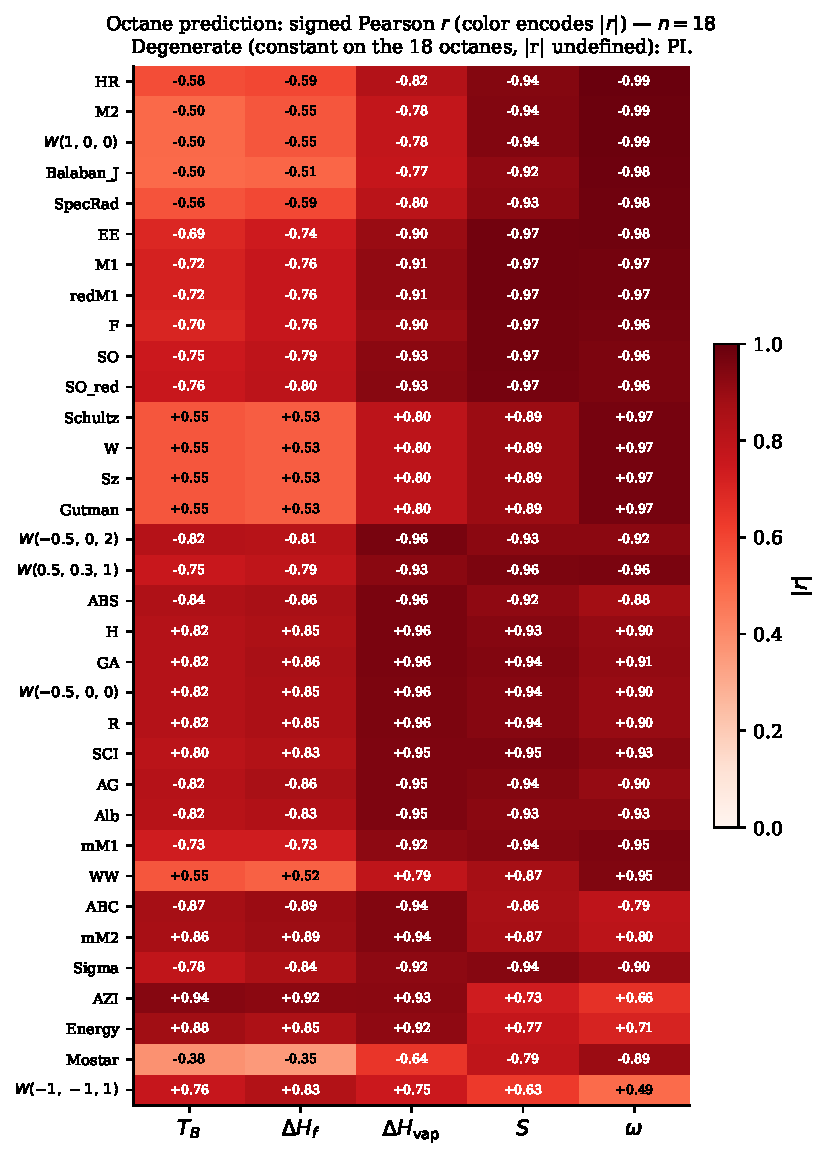
\includegraphics[width=0.95\linewidth]{fig4_octane_heatmap.pdf}
\caption{Signed Pearson $r$ between each Wuzi/classical index and
each of 8 octane properties (18 isomers). Color encodes $|r|$;
values are printed with sign. $PI$ is degenerate on the dataset and
removed (Remark~\ref{rem:pi_octanes}).}
\label{fig:octanes}
\end{figure}

\subsection{Degeneracy on trees of order 10}\label{sec:degeneracy}

Following~\cite{MovahediGutmanRedzepovicFurtula2026} Section~5.3,
we report the degeneracy (fraction of indistinguishable structures)
of each index on the $106$ non-isomorphic trees of order~$10$.
Wuzi values at $\gamma=2$ achieve $\sim25\%$ degeneracy, comparable
to the Sombor-family range $17$--$22\%$ reported
in~\cite{MovahediGutmanRedzepovicFurtula2026} Figure~5.

\begin{figure}[h]
\centering
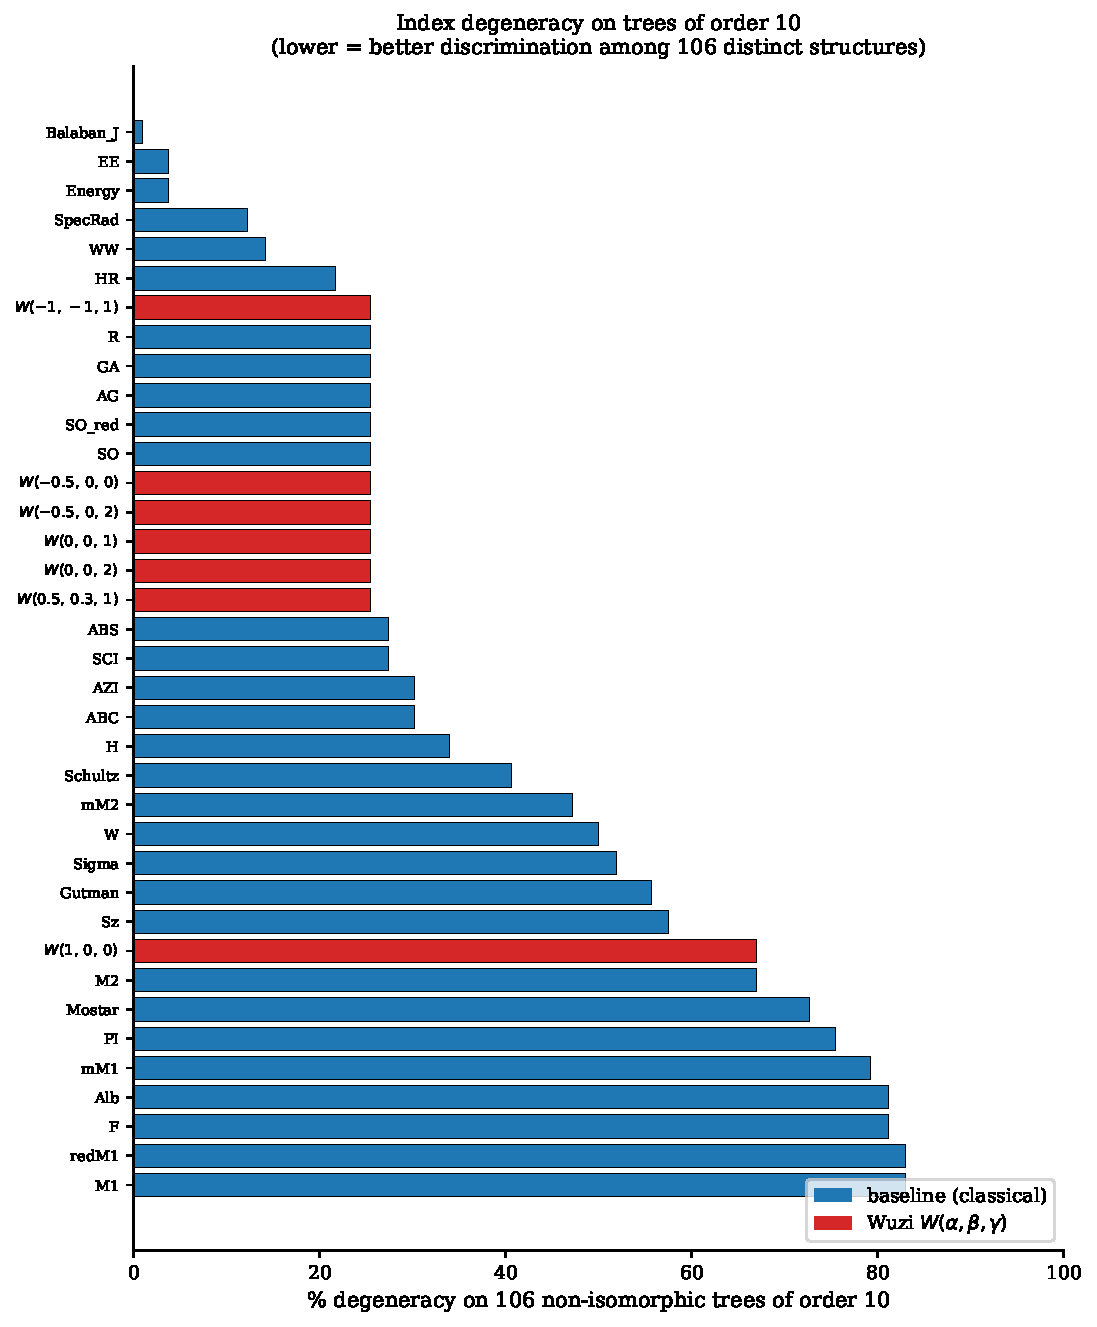
\includegraphics[width=0.85\linewidth]{fig6_degeneracy_bars.pdf}
\caption{Percent degeneracy on $106$ non-isomorphic trees of order
$10$ for each of the $30$ baseline indices and selected Wuzi
parameter points.}
\label{fig:degeneracy}
\end{figure}

\subsection{Structure sensitivity on decane isomers}\label{sec:ss}

Following~\cite{MovahediGutmanRedzepovicFurtula2026} Section~5.4,
we compute the structure-sensitivity metrics
$SS=\sigma/\mu, \; Abr=(\max-\min)/\mu, \; SA=SS/Abr$
on the $75$ decane isomers (Fig.~\ref{fig:ss}). Wuzi values lie in
the same regime as the Sombor variants reported
in~\cite{MovahediGutmanRedzepovicFurtula2026} Table~2.

\begin{figure}[h]
\centering
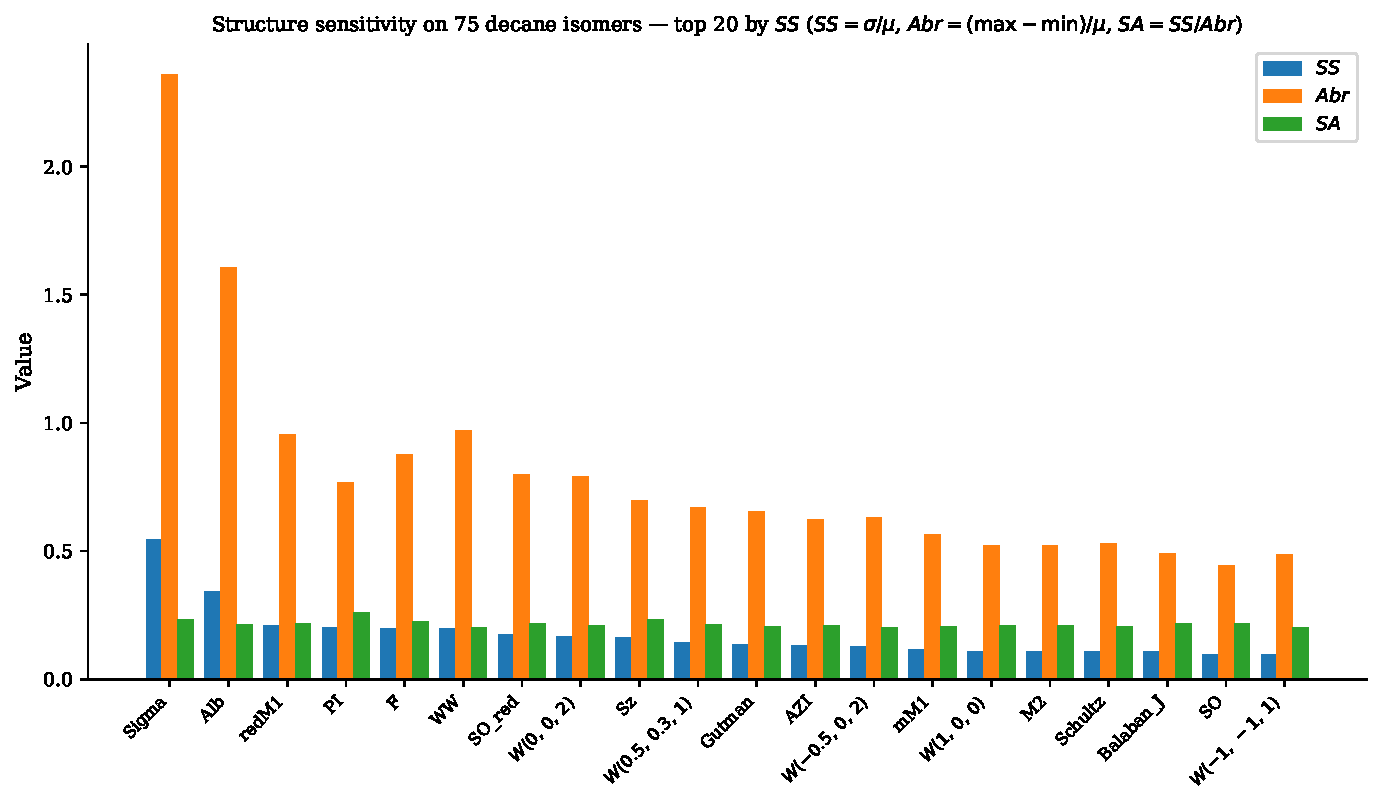
\includegraphics[width=0.95\linewidth]{fig7_structure_sensitivity.pdf}
\caption{Structure-sensitivity metrics on the $75$ decane isomers,
top $20$ indices by $SS$.}
\label{fig:ss}
\end{figure}

% =====================================================================
\section{Discussion}\label{sec:discussion}
% =====================================================================

The Wuzi family is structurally rich (Sections~\ref{sec:closedforms}--\ref{sec:psi}):
it admits closed-form values on nine standard graph classes,
recovers $M_2,R,\chi,H$ as special cases, and admits a bracket
bound via the edge-contribution function that becomes an exact
identity on regular graphs.

At the same time the sensitivity behaviour on the standard
math-chem benchmarks (Section~\ref{sec:sensitivity}) is
competitive with established BID indices on a subset of the
octane physicochemical properties (notably $\Delta H_\mathrm{vap}$
and $\omega$) and structurally interpretable on the trees-of-order-10
degeneracy and the decane structure sensitivity. We do not claim
the family is uniformly superior to any classical index on any
benchmark; the comparison is sensitivity-only.

The combination of structural and empirical observations supports a
careful reading: the Wuzi family is a meaningful object of study on
the mathematical side (closed forms, bounds, and extremal graphs in
the classical tradition); on the chemometric side it provides a
transparent worked example of a parametric BID generalization at
the same correlation regime as established indices. The
BID-basis observation of Theorem~\ref{thm:bid} explicitly accounts
for the family's inability to escape the $10$-dimensional BID
subspace on $\mathcal{G}_4$; the multi-dataset redundancy
screening of the family and the downstream predictive-model
benchmark are reported in the companion methodology
paper~\cite{Paper2_Screening}.

\paragraph{Future work.} The mathematical program of
Sections~\ref{sec:bounds_nm}--\ref{sec:extremal} is partially
complete; the [PROOF SKETCH] markers indicate the formal results
that remain to be derived. Specifically:
\begin{enumerate}
\item Sharp Nordhaus--Gaddum bounds for $\Wuzi(G)+\Wuzi(\bar G)$
(Theorem~\ref{thm:NG}).
\item Tight bounds via $SO,\,GA,\,H,\,ABC$ in the full
$(\alpha,\beta,\gamma)$ region (Theorems~\ref{thm:sombor}--\ref{thm:H_ABC}).
\item Formal extremal-graph characterization for trees, unicyclic,
and bicyclic graphs in every parameter sign region
(Conjectures~\ref{conj:trees_beta_pos}--\ref{conj:bicyclic}).
\item Closed-form bounds involving the Albertson irregularity
$\mathrm{Alb}(G)=\sum_e|d_u-d_v|$, naturally paired with the
Wuzi $\gamma$-axis.
\end{enumerate}

On the chemometric side, future work includes extending the
sensitivity-analysis benchmarks to additional compound classes
(benzene derivatives, alkane homologues beyond octane / decane)
and to compound-class-specific QSPR endpoints. The
methodology-paper side of the analysis (multi-dataset
orthogonality screening, downstream ML benchmark, partial-
correlation sensitivity to thresholds) is reported separately
in~\cite{Paper2_Screening}.

% =====================================================================
\section{Conclusion}\label{sec:conclusion}
% =====================================================================

We have introduced the Wuzi index family $\Wuzi$ and (i) derived
closed-form values on nine standard graph classes, (ii) established
a bracket bound via the edge-contribution function, with the
bracket being tight on regular graphs, (iii) given exact reductions
to classical indices $M_2, R, \chi, H$ at six parameter points,
(iv) proved a rigorous ratio-bound theorem for the family against
any classical BID index with strictly positive edge contribution,
and (v) reported sensitivity analysis on the $18$ octane isomers,
on the $106$ non-isomorphic trees of order $10$, and on the $75$
decane isomers, showing the family is in the same correlation
regime as established BID indices on the standard math-chem
benchmarks. The Edge-Degree-Pair Basis observation gives a
$10$-dimensional ceiling on the BID family on $\mathcal{G}_4$ and
underlies the multi-dataset screening behaviour reported in the
companion methodology paper~\cite{Paper2_Screening}.

The formal bounds in $(n,m,\Delta,\delta)$ and via classical
indices, as well as the extremal-graph characterizations for
trees, unicyclic, and bicyclic graphs, are partially complete in
the present draft; the remaining derivations are reserved for
joint work with the senior author.

% =====================================================================
\section*{Data and code availability}
% =====================================================================

All numerical computations, code, datasets (or download scripts),
and figures are publicly available at
\url{https://github.com/Singati2/topological-index-orthogonality}.
The reference implementation runs end-to-end in well under a
minute on a single laptop.

% =====================================================================
\section*{Acknowledgements}
% =====================================================================

The authors thank colleagues for discussions of the computational
extremal-graph search and the redundancy-screening protocol.
Funding sources and institutional support to be acknowledged in
the final version of the manuscript.

% =====================================================================
\begin{thebibliography}{99}
% =====================================================================
\small

\bibitem{Wiener1947}
H.~Wiener,
\emph{Structural determination of paraffin boiling points},
J.~Am.~Chem.~Soc.~\textbf{69} (1947), 17--20.

\bibitem{Randic1975}
M.~Randi\'c,
\emph{On characterization of molecular branching},
J.~Am.~Chem.~Soc.~\textbf{97} (1975), 6609--6615.

\bibitem{Gutman1972}
I.~Gutman and N.~Trinajsti\'c,
\emph{Graph theory and molecular orbitals. Total
$\pi$-electron energy of alternant hydrocarbons},
Chem.~Phys.~Lett.~\textbf{17} (1972), 535--538.

\bibitem{Fajtlowicz1987Harmonic}
S.~Fajtlowicz,
\emph{On conjectures of Graffiti-II},
Congr.~Numer.~\textbf{60} (1987), 187--197.

\bibitem{ZhouTrinajstic2009sumconn}
B.~Zhou and N.~Trinajsti\'c,
\emph{On a novel connectivity index},
J.~Math.~Chem.~\textbf{46} (2009), 1252--1270.

\bibitem{BollobasErdos1998}
B.~Bollob\'as and P.~Erd\H{o}s,
\emph{Graphs of extremal weights},
Ars Combin.~\textbf{50} (1998), 225--233.

\bibitem{Gutman2021Sombor}
I.~Gutman,
\emph{Geometric approach to degree-based topological indices: Sombor indices},
MATCH Commun.~Math.~Comput.~Chem.~\textbf{86} (2021), 11--16.

\bibitem{MovahediGutmanRedzepovicFurtula2026}
F.~Movahedi, I.~Gutman, I.~Red\v{z}epovi\'c, and B.~Furtula,
\emph{Diminished Sombor index of graphs},
MATCH Commun.~Math.~Comput.~Chem.~\textbf{95} (2026), 141--162.

\bibitem{Movahedi2025arXivDSO}
F.~Movahedi,
\emph{Bounds for the Diminished Sombor index of graphs},
arXiv preprint, 2025. \todo{[VOL/ID REFERENCE NEEDED]}

\bibitem{GutmanBorovicanin2018BID}
I.~Gutman and B.~Borovi\'canin,
\emph{Edge-degree-based topological indices and their applications}
(survey paper), \todo{[FULL CITATION REFERENCE NEEDED]}.

\bibitem{HardyLittlewoodPolya1934}
G.~Hardy, J.~E.~Littlewood, and G.~P\'olya,
\emph{Inequalities},
Cambridge University Press, 1934.

\bibitem{GutmanFurtulaBook2017}
I.~Gutman and B.~Furtula (eds.),
\emph{The Randi\'c Index: Theory and Applications},
\todo{[PUBLISHER / YEAR REFERENCE NEEDED]}.

\bibitem{HansenMelot2003unicyclicRandic}
P.~Hansen and H.~M\'elot,
\emph{Variable neighborhood search for extremal graphs},
\todo{[FULL CITATION REFERENCE NEEDED]}.

\bibitem{HansenMelot2005bicyclicBounds}
\todo{[BICYCLIC EXTREMAL REFERENCE NEEDED]}.

\bibitem{NordhausGaddumOrig1956}
E.~A.~Nordhaus and J.~W.~Gaddum,
\emph{On complementary graphs},
Amer.~Math.~Monthly~\textbf{63} (1956), 175--177.

\bibitem{Paper2_Screening}
G.~Shiwakoti, A.~Natarajan, M.~Arockiaraj,
\emph{Orthogonality Screening of Topological Indices for QSPR Modeling:
A Reproducible Pipeline and Software Framework},
in preparation, 2026.
(Companion methodology paper.)

\end{thebibliography}
\end{document}
